\documentclass[spanish]{article}

%%%%%%%%%%%%%%%%%%%%%%%%%%%%%%%%%%%%%%%%%%%%%%%%%%%%%%%%%%%%%%%%%%%%%%%%%%%%%%%%

% Language
\usepackage[spanish]{babel}

% Support for images
\usepackage{graphicx}

% Underlining
\usepackage{amsmath}

% Avoiding indenting of first paragraph's line.
\setlength{\parindent}{0cm}

% Support for hyperlinks.
\usepackage{hyperref}
\hypersetup {
        linktoc=all,
        hidelinks
}

% Additional section formatting.
\renewcommand\thesection{\arabic{section}}
\renewcommand\thesubsection{\thesection.\arabic{subsection}}

% Cover of the document
\title{Sistemas Operativos - Práctica 2}
\author{Oussama Akachach Jouhrati\\
[0.5cm]{\small Profesor/a: Montserrat Ferrer Serafí}}
\date{\today}

%%%%%%%%%%%%%%%%%%%%%%%%%%%%%%%%%%%%%%%%%%%%%%%%%%%%%%%%%%%%%%%%%%%%%%%%%%%%%%%%

\begin{document}

\pagenumbering{gobble}
\maketitle
\newpage

\tableofcontents
\pagenumbering{arabic}
\setcounter{page}{2}

\newpage

% Customize from here.

\section{Pregunta 1}

\subsection{}

\subsubsection{}

Se trata de un programa que, recursivamente, va generando
procesos hijo. Cada uno de estos procesos, una vez
completado, escriben en la consola su número de proceso y el
valor del contador el bucle (variable) que tengan
registrado. Seguido de ello, se finalizan a ellos mismos,
mediante la función exit(0).\\

El bucle recursivo sigue la siguiente lógica:\\

\textbf{Creamos el proceso padre P1}

\begin{itemize}
\item P1: n = 0
\item P1: entramos en el bucle.
\item P1: generamos el proceso P2 (n = 0)

\item P2: aumentamos n (n = 1)
\item P2: en el if, aumentamos n de nuevo, puesto que pid
será igual a nuestro número de proceso (n = 2).
\item P2: generamos el proceso P3 (n = 2).

\item P3: aumentamos n (n = 3)
\item P3: en el if, aumentamos n de nuevo, puesto que pid
será igual a nuestro número de proceso (n = 4).
\item P3: \textbf{Escribimos a la consola: Result process:
P3: 4.}
\item P3: Escribimos lo mismo en el file descriptor 1.
\item P3: terminamos el proceso P3.

\item P2: generamos el proceso P4 (n = 3).

\item P4: aumentamos n (n = 4).
\item P4: en el if, aumentamos n de nuevo, puesto que pid
será igual a nuestro número de proceso (n = 5).
\item P4: \textbf{Escribimos a la consola: Result process:
P4: 5.}
\item P4: Escribimos lo mismo en el file descriptor 1.
\item P4: terminamos el proceso P4.

\item P2: aumentamos n (n = 4).
\item P2: en el if, esperamos a que el proceso P4 acabe,
puesto que pid será igual a 0, ya que es el valor de retorno
de la función fork() para el proceso padre.
\item \textbf{Escribimos a la consola: Result process: P2:
4.}
\item Escribimos lo mismo en el file descriptor 1.
\item Terminamos el proceso P2.

\item P1: aumentamos n (n = 1)
\item P1: en el if, esperamos a que el proceso P2 acabe,
puesto que pid será igual a 0, ya que es el valor de retorno
de la función fork() para el proceso padre.
\item P1: generamos el proceso P5.

\item P5: aumentamos n (n = 2).
\item P5: en el if, aumentamos n de nuevo, puesto que pid
será igual a nuestro número de proceso (n = 3).
\item P5: generamos el proceso P6.

\item P6: aumentamos n (n = 4).
\item P6: en el if, aumentamos n de nuevo, puesto que pid
será igual a nuestro número de proceso (n = 5).
\item P6: \textbf{Escribimos a la consola: Result process:
P6: 5.}
\item P6: Escribimos lo mismo en el file descriptor 1.
\item P6: Terminamos el proceso P6.

\item P5: aumentamos n (n = 4).
\item P5: en el if, esperamos a que el proceso P6 acabe,
puesto que pid será igual a 0, ya que es el valor de retorno
de la función fork() para el proceso padre.
\item P5: \textbf{Escribimos a la consola: Result process:
P5: 4.}
\item P5: escribimos lo mismo en el file descriptor 1.
\item P5: terminamos el proceso P5.

\item P1: aumentamos n (n = 2).
\item P1: en el if, esperamos a que el proceso P5 acabe,
puesto que pid será igual a 0, ya que es el valor de retorno
de la función fork() para el proceso padre.
\item P1: generamos el proceso P7.

\item P7: aumentamos n (n = 3).
\item P7: en el if, aumentamos n de nuevo, puesto que pid
será igual a nuestro número de proceso (n = 4).
\item P7: \textbf{Escribimos a la consola: Result process:
P7: 4.}
\item P7: escribimos lo mismo en el file descriptor 1.
\item P7: terminamos el proceso P7.

\item P1: aumentamos n (n = 3).
\item P1: en el if, esperamos a que el proceso P7 acabe,
puesto que pid será igual a 0, ya que es el valor de retorno
de la función fork() para el proceso padre.
\item P1: generamos el proceso P8.

\item P8: aumentamos n (n = 4).
\item P8: en el if, aumentamos n de nuevo, puesto que pid
será igual a nuestro número de proceso (n = 5).
\item P8: \textbf{Escribimos a la consola: Result process:
P8: 5.}
\item P8: escribimos lo mismo en el file descriptor 1.
\item P8: terminamos el proceso P8.

\item P1: aumentamos n (n = 4).
\item P1: en el if, esperamos a que el proceso P8 acabe,
puesto que pid será igual a 0, ya que es el valor de retorno
de la función fork() para el proceso padre.
\item P1: \textbf{Escribimos a la consola: Result process:
P1: 4.}
\item P1: escribimos lo mismo en el file descriptor 1.
\item P1: terminamos el proceso P1.

\end{itemize}

\newpage

La salida estándar será la equivalente:\\

Result process: P3: 4.\\

Result process: P4: 5.\\

Result process: P2: 4.\\

Result process: P6: 5.\\

Result process: P5: 4.\\

Result process: P7: 4.\\

Result process: P8: 5.\\

Result process: P1: 4.\\

Y la salida del código es:

\begin{center}
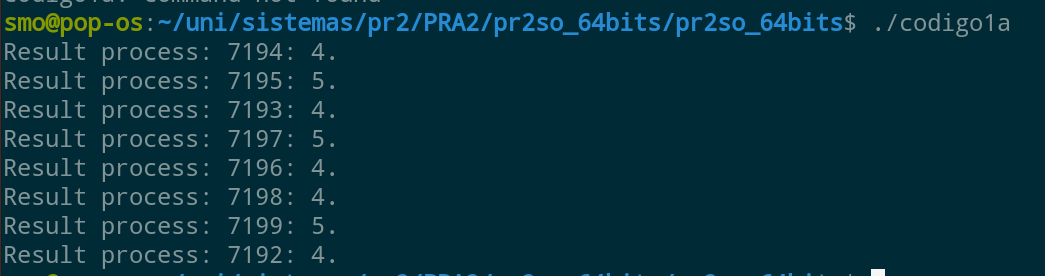
\includegraphics[width=12cm]{../img/1.png}
\end{center}

Contando el proceso padre, se generan en total 8 procesos.

\newpage

\subsubsection{}

Este código representa la comunicación entre dos procesos:
el padre y el hijo.\\

Inicialmente, establecemos dos canales (pipes) para la
comunicación entre estos dos procesos. Necesitamos dos,
puesto que las pipes son unidireccionales, es decir, que
sólo uno de los lados puede leer o escribir.\\

Generamos un proceso hijo a partir del proceso padre y se
realizan las siguientes operaciones ``simultáneamente'':

\begin{itemize}
\item Proceso padre: escribe en el file descriptor establecido por
el primer pipe (p[0]) el valor de la variable pid, que en
este caso, será el número del proceso hijo.

\item Proceso hijo: escribe en el file descriptor
establecido por el segundo pipe (p[1]) el valor de la
variable pid, que en este caso, será el número 0, que es el
valor de retorno de la función fork() para el proceso hijo.

\item Proceso padre: lee en el file descriptor establecido
por el segundo pipe (p[1]) el valor de la variable pid, que
en este caso, será el número del proceso hijo.

\item Proceso hijo: lee en el file descritor establecido por
el primer pipe (p[1]) el valor de la variable pid, que en
este caso, será el número 0, puesto que es el valor de
retorno de la función fork() para el proceso hijo.

\end{itemize}

En caso de que se trate del proceso padre, esperaremos a que
termine el proceso hijo para proceder. Aquí, este escribirá
en la consola \textbf{Result process PH: 0}, ya que el valor
de pid que tendrá será el devuelto por la función fork().\\

Escribirá el mismo mensaje en el file descriptor 1 y
se finalizará a si mismo.\\

Al terminar el proceso hijo, el padre hará lo mismo, pero su
valor de pid corresponderá al número de proceso del hijo, ya
que ese es el valor devuelto por la función fork() para el
proceso padre.\\

Escribirá el mismo mensaje en el file descriptor 1 y se
finalizará a si mismo.\\

\textbf{Output esperado:}\\

Result process PH: 0.\\

Result process PP: PH.\\

\begin{center}
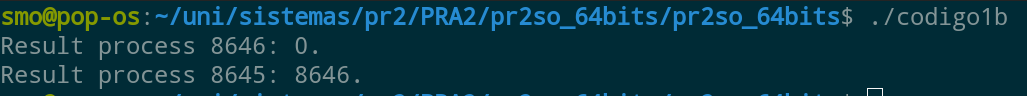
\includegraphics[width=12cm]{../img/2.png}
\end{center}

\subsection{}

\subsubsection{}

En este programa utilizamos el sigaction siga para modificar
el comportamiento de la señal SIGINT. Se establece como
static struct para que su valor se tenga en cuenta en todo
el programa, y no sólo en la función main().\\

Establecemos a cero el valor de la variable siga mediante la
función bzero, y seguido de ello, vinculamos la función
Handler al sigaction siga. De esta manera, cuando vinculemos
una señal al sigaction y esta sea enviada, se ejecutará la
función Handler().\\

Seguido de ello, vinculamos la señal SIGINT al sigaction
siga mediante la función SIGACTION. Al ser nulo el tercer
argumento, sólo se ejecutará la función que hayamos
vinculado en el sigaction siga (la función Handler).\\

Creamos un proceso hijo mediante la función fork() y
guardamos el resultado en la variable pid.\\

Para el proceso padre, pid será igual al proceso hijo,
mientras que para el proceso hijo, pid será igual a 0.\\

Mediante la función kill, enviamos la señal SIGINT al número
de proceso que tengamos almacenado en nuestra variable pid.
Si se trata del proceso padre, este enviará la señal SIGINT
al proceso hijo, ejecutando la función Handler por su parte
y al hijo, incrementando para ambos el valor de la variable
count en 1 (count = 1 para ambos) y esperará a que el
proceso hijo termine, mediante la función wait(NULL).\\

Cabe decir que la función kill() no detendrá el proceso para
ninguno de los dos procesos, puesto que hemos vinculado la
señal SIGINT a la función Handler para los dos procesos,
mediante el sigaction().\\

Por parte del proceso hijo, se volverá a ejecutar la función
kill(), con pid = 0, puesto que ese es el valor de retorno
de la función fork() para el proceso hijo, enviando la señal
SIGINT a todos los procesos del mismo grupo (él mismo y sus
hijos). Como el proceso hijo no tiene procesos hijos, se
enviará la función SIGINT únicamente a sí mismo, activando
de nuevo la función Handler, y sumándo una unidad a su
versión de la variable count (count = 2).\\

En la función wait(), el proceso hijo no tendrá que esperar,
puesto que no tiene procesos hijo ejecutándose.\\

El proceso hijo enviará el siguiente mensaje a la consola:
\textbf{Result process PH: 2}, ya que éste es su valor de la
variable count. Hará lo mismo para el file descriptor 1 y
terminará el proceso.\\

Una vez termine, el proceso padre hará lo mismo, escribiendo
en la consola: \textbf{Result process PP: 1}, ya que éste es
su valor de la variable count. Hará lo mismo para el file
descriptor 1 y terminará el proceso.\\

\textbf{Resultado esperado:}\\

Result process PH: 2.\\

Result process PP: 1.\\

\textbf{Resultado obtenido:}\\

\begin{center}
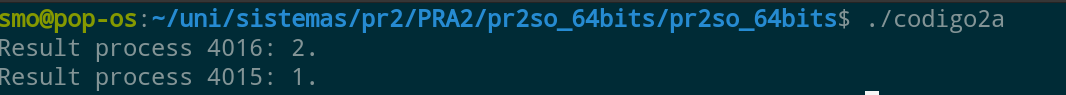
\includegraphics[width=12cm]{../img/3.png}
\end{center}

\subsubsection{}

Este programa tiene un comportamiento similar al anterior,
pero en este caso, la señal que estamos vinculando con la
misma función Handler() es la señal SIGKILL.\\

Hay que tener en cuenta que la señal SIGKILL no se puede
vincular con nada, ya que siempre terminará el programa.\\

Teniendo eso en cuenta y una vez realizada la vinculación, generamos un proceso hijo
y, en caso de que en la ejecución del programa se trate del
proceso hijo, se ejecutará el comando ``sleep 10'', mediante
la función execlp. Si todo va bien, no deberían ejecutarse
las líneas posteriores del programa para el código hijo,
puesto que execlp() sustituye la ejecución del programa del
proceso sobre el cual se esté ejecutando por lo que se haya
introducido como argumentos.\\

Para el proceso padre, enviaremos la señal SIGKILL para el pid
del proceso hijo, donde se terminará el proceso del comando,
sin ejecutar su función Handler. Lo mismo pasará para el
proceso padre, pero este no detendrá su ejecución, puesto
que hemos enviado dicha señal exclusivamente al pid del
proceso hijo.\\

El proceso padre tendrá que esperar a que el proceso hijo
termine, por la función wait(). En este caso, no tendrá que
esperar nada, ya que el proceso hijo se ha terminado en la
línea anterior, con la función kill() enviada.

El proceso padre escribirá en la consola: \textbf{Result
process PP: 0}. Hará lo mismo para el file descriptor 1 y
terminara su proceso. La variable count sigue valiendo 0
porque en ningún momento se ha entrado en la función
Handler, ya que, como hemos dicho antes, la señal SIGKILL no
se puede vincular con nada.\\

\textbf{Resultado esperado:}

Result process PP: 0.\\

\textbf{Resultado obtenido:}

\begin{center}
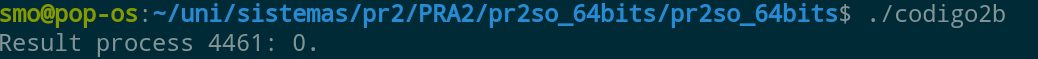
\includegraphics[width=12cm]{../img/4.png}
\end{center}

\section{Pregunta 2}

\subsection{}

\subsubsection{}

El contenido de esta sección está en los archivos
WordCount\_2-1.c y WordCount\_Child\_2-1.c.

\subsubsection{}

Los resultados son diferentes debido a que, en nuestro caso,
estamos utilizando el código de finalización del proceso
como valor de salida para el resultado del recuento de
carácteres. Este proceso funcionará correctamente siempre y
cuando el recuento no llegue a más de 255 unidades, puesto
que los códigos de finalización van de 0 a 255.\\

Para poder solucionar este problema, podemos implementar una
solución en la que utilicemos pipes como método de
comunicación entre procesos, en lugar de utilizar el código
de finalización del proceso. Se enviaría el valor del
recuento, escribiendo el lado del proceso hijo y leyendo en
el lado del proceso padre.

\subsection{}

\subsection{}

\subsection{}


\newpage

\begin{thebibliography}{X}

\end{thebibliography}

\end{document}
